\section{Conception}

This section will detail the conception and the class diagram of our project. The following graphic shows the different classes we used in the project.

\begin{figure}[H]
 \centering
 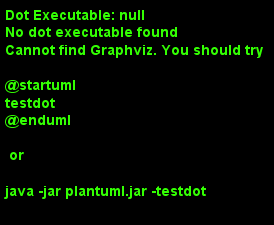
\includegraphics[scale=0.5]{../uml/classDiagram.png}
 \caption{Class diagram}
\end{figure}

\subsection{StaticGesture and StaticGestures}

StaticGesture (without s) is not really a class, it is an enum that holds all of the static gestures that are possible to detect. The main aim of using an enum here is to avoid having to handle the value of each gesture and make it more user friendly.

StaticGestures (with an s) is the class which allow the user to detect the StaticGesture within a frame. To make the program run faster a simple set of hand (Leap::HandList) is required when the object is created. A new object is required to be created each time a new HandList is used. This last part is one of the possible improvement on the code (even if the creation of the new object make sense and is viable).

\subsection{GestValidator}

As far as StaticGestures is concerned, a new gesture is possibly detected after each new frame. Since this is not usable for the user, the class GestValidator was added. This class allows to set a number of frame on which the gesture needs to be in order to be validated.
Within this class, two functions need to be detailed : "update" and "setGesture". Their aim may seem identical even if they are not, the "update" function allows the user to update the gesture within the GestValidator object i.e 11th gesture is CLOSED\_HAND. Whereas the "setGesture" function sets the gesture count to 0 i.e 1st gesture is now CLOSE\_HAND (and if the "update" function is used after that we have the 2nd gesture count is 2, 3,...).

\subsection{DetectionListener}

This class is one of the simplest one, it is one of the class given within the LeapMotion api, it allows the user to define what will happen when a certain event is triggered.
Here we use it to handle the mode selection (static or dynamic) and to update the detection of the gesture.

\subsection{ModeHandler}

This is the class used to handle the different mode which are available within the program (static and dynamic). The user only needs to call the function modeX to process the required mode. The class will manage the communication with the robot through the Communicator (see below). Each previous state is stored and this class should not be re-instansciated after each new frame.

It is within this class that the filter is used (dynamic mode) in order to smoothen the output when communicating with the robot.

\subsection{Communicator}

This is the class that handles the TCP communication. It is a simple class which will connect to the robot and then send the data through the function sendData(). This last function allows the user to set a delay or not in order to give the robot some time to carry out the action that is required.
